\documentclass[tikz,border=7pt]{standalone}
\usepackage{amsmath}
\usetikzlibrary{arrows.meta,decorations.pathmorphing}

\definecolor{ink}{HTML}{21352F}
\definecolor{teal}{HTML}{087F7B}
\definecolor{rose}{HTML}{B65A62}
\definecolor{gold}{HTML}{C58B2A}
\definecolor{blue}{HTML}{4B77A8}

\begin{document}
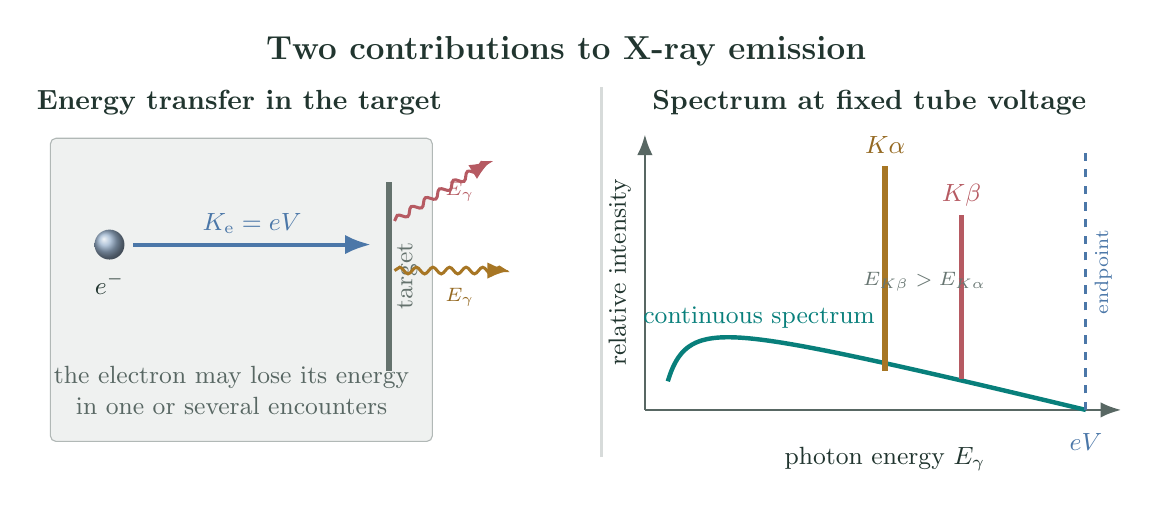
\begin{tikzpicture}[font=\sffamily,>=Latex]
  \node[font=\bfseries\large,text=ink] at (0,2.8)
    {Two contributions to X-ray emission};

  % Tube-energy panel
  \node[font=\bfseries,text=ink] at (-4.15,2.15)
    {Energy transfer in the target};
  \draw[rounded corners=2pt,fill=ink!7,draw=ink!35]
    (-6.55,-2.15) rectangle (-1.7,1.7);
  \draw[line width=2.3pt,draw=ink!70] (-2.25,-1.25) -- (-2.25,1.15);
  \node[rotate=90,text=ink!70,font=\small] at (-2.02,-0.05) {target};

  \shade[ball color=blue!55] (-5.8,0.35) circle (0.19);
  \node[text=ink,font=\small] at (-5.8,-0.15) {$e^-$};
  \draw[->,line width=1.4pt,draw=blue]
    (-5.5,0.35) -- (-2.48,0.35)
    node[midway,above,text=blue,font=\small] {$K_{\mathrm e}=eV$};

  \draw[->,decorate,decoration={snake,amplitude=1.2pt,segment length=6pt},
        line width=1.1pt,draw=rose]
    (-2.18,0.65) -- (-0.95,1.42);
  \draw[->,decorate,decoration={snake,amplitude=1.2pt,segment length=6pt},
        line width=1.1pt,draw=gold!85!black]
    (-2.18,0.02) -- (-0.72,0.02);
  \node[text=rose,font=\scriptsize] at (-1.35,1.02) {$E_\gamma$};
  \node[text=gold!75!black,font=\scriptsize] at (-1.35,-0.32)
    {$E_\gamma$};
  \node[align=center,text=ink!75,font=\small] at (-4.25,-1.5)
    {the electron may lose its energy\\in one or several encounters};

  \draw[ink!18,line width=1pt] (0.45,-2.35) -- (0.45,2.35);

  % Spectrum panel
  \node[font=\bfseries,text=ink] at (3.85,2.15)
    {Spectrum at fixed tube voltage};
  \draw[->,line width=1pt,draw=ink!75]
    (1.0,-1.75) -- (7.05,-1.75);
  \node[below=10pt,text=ink,font=\small] at (4.05,-1.75)
    {photon energy $E_\gamma$};
  \draw[->,line width=1pt,draw=ink!75]
    (1.0,-1.75) -- (1.0,1.75);
  \node[rotate=90,text=ink,font=\small] at (0.68,0)
    {relative intensity};

  % A smooth qualitative continuum with an exact endpoint at E_gamma=eV.
  \draw[line width=1.6pt,draw=teal,domain=0.14:5.45,samples=120,smooth,
        variable=\x]
    plot ({1.15+\x},
      {-1.75+1.35*(1-\x/5.45)*exp(-0.18/\x)});
  \node[text=teal,font=\small] at (2.45,-0.58)
    {continuous spectrum};

  % Characteristic spikes: K beta has the larger photon energy.
  \draw[line width=2pt,draw=gold!85!black] (4.05,-1.25) -- (4.05,1.35);
  \draw[line width=2pt,draw=rose] (5.02,-1.36) -- (5.02,0.72);
  \node[text=gold!75!black,font=\small] at (4.05,1.62) {$K\alpha$};
  \node[text=rose,font=\small] at (5.02,0.98) {$K\beta$};
  \node[text=ink!68,font=\scriptsize,align=center] at (4.55,-0.12)
    {$E_{K\beta}>E_{K\alpha}$};

  \draw[dashed,draw=blue,line width=1pt] (6.6,-1.75) -- (6.6,1.52);
  \node[below=5pt,text=blue,font=\small] at (6.6,-1.75) {$eV$};
  \node[rotate=90,text=blue,font=\scriptsize] at (6.82,0.0)
    {endpoint};
\end{tikzpicture}
\end{document}
